\documentclass[11pt,twoside,a4paper]{article}
\usepackage[utf8]{inputenc}
\usepackage{amsmath}
\usepackage{amsfonts}		
\usepackage{amssymb}
\usepackage{graphicx}
\usepackage{url}
\usepackage{mathrsfs}
\usepackage{multicol}
\usepackage{tikz}
\usepackage{amsthm}
\usepackage{hyperref}
\usepackage{natbib}
\usepackage{caption}
\usepackage{subcaption}
\renewcommand{\bibsection}{}
\usetikzlibrary{arrows}
\usetikzlibrary{positioning}
\tikzset{>=latex}
\usepackage{verbatim}
\usepackage[margin=2cm]{geometry}
\newcommand*\diff{\mathop{}\!\mathrm{d}}
\author{Eleanor McMurtry\\760505}
\title{Building a magneto-optical trap for rubidium atoms: a practical guide for the intrepid third year}
\begin{document}
\maketitle
\section*{Abstract}
Our goal for this project was to develop a procedure by which third-year undergraduate students could
build, test, and experiment with a magneto-optical trap (MOT) for rubidium-85 atoms. Our setup used an external-cavity diode laser (ECDL)
split into three arms with retro-reflection, and an additional ECDL used as a repumping beam.
We successfully constructed a MOT and demonstrated its effectiveness, though our setup required the use of expensive and fiddly fibre optic couples.
These were chosen for flexibility; an implementation of the experiment would need only minor modifications
to avoid using these.

This document is intended to be both a reflection of our experiences and a guide for a prospective
third year laboratory experiment. I will first outline some of the relevant theory for the experiment,
then discuss the experimental procedures required to build the MOT;\@ I will conclude the document with a brief
discussion of our results, followed by an outline of ways to extend the experiment.

\begin{center}    
\subsection*{Supervised by Andy McCulloch and Robert Scholten}
University of Melbourne School of Physics\\
Thanks also to Alexander Wood for his tireless assistance in the lab.
\end{center}
\pagebreak
\tableofcontents
\vfill
\pagebreak
\section{Introduction}
Optical trapping methodologies have their origin in the 1970s, when~\cite{ashkin1970} developed what has become known
as optical tweezers using electromagnetic gradients. Following this was a flurry of research, on both refining this method
as well as entirely novel approaches to creating optical traps. Laser cooling -- one of the techniques used in MOTs -- was
first demonstrated by~\cite{wineland1978}, who were able to cool Mg (II) ions to temperatures below 40 K. This method was improved
upon by~\cite{chu1985}, cooling atoms to \(\sim240 \operatorname{\mu}\)K with ``optical molasses'', using a laser slightly detuned from resonance.
Atoms moving towards the laser see a Doppler-shifted beam closer to resonance, and therefore are more likely to interact with the beam.
\\\\
Magneto-optical traps take laser-cooled atoms, and apply a magnetic quadrupole to take advantage of the Zeeman effect. By
introducing a radially-increasing field, the magnetically-sensitive energy levels are shifted closer to the laser's resonance as the atom moves
from the trap's centre. By this mechanism, explored in further detail in Section 2, atoms are trapped in the centre of the
apparatus. The first such trap was constructed by~\cite{raab1987}, who were able to confine and cool a cloud of neutral sodium atoms. For this and related
work, the 1997 Nobel Prize in Physics was awarded to several of the relevant researchers.
\\\\
Alkali metals are the preferred atoms of choice for magneto-optical trapping due to their hydrogenic atomic structure; they can be approximated
as a simple two-state atom. Rubidium atoms in particular are popular due to their convenient atomic structure, and the fact that their transition frequencies
are in the range of cheap and readily available diode lasers at approximately 780nm.
\\\\
To achieve the precision required for laser cooling, we used saturated absorption spectroscopy. Since atoms in a vapour cell have a distribution of velocities,
incident light will be Doppler shifted differently for various atoms in the sample. This limits the precision of absorption measurements not by the fundamental width
of the transition, but instead by this Doppler broadening effect. To overcome this issue, a retro-reflected laser (called the probe beam) is recorded instead. By saturating the sample,
the probe beam will interact with far fewer atoms when it is on resonance with the hyperfine transitions, resulting in sharp dips in the Doppler-broadened peaks at the resonant frequencies.
In this way, the hyperfine splitting of rubidium-85 in the \(5P_{3/2}\) state can be revealed. By setting the lasers in the vicinity of the appropriate transitions and fine-tuning the frequency,
we were able to demonstrate our MOT.\@
\vfill
\pagebreak
\section{Background theory}
\subsection{Doppler cooling}
On a macroscopic scale, the most familiar reaction to a laser pointed at a material is for the material to heat up due to the energy transferred from the photons to the material. On a microscopic scale,
however, the interaction is subtler, and this can lead to wildly different behaviour. Doppler cooling is one such example.

Consider a simple two-state atom of mass \(m\), with a transition from a ground state to an excited state at frequency \(f\). Take a photon with momentum \(p=\frac{hf}{c}\) in direction \(\vec{\hat{v}}\), where \(h\) is Planck's constant, and \(c\) is the speed of light.
If this photon is incident on the atom it can be absorbed to bring the atom to
its excited state, and thus cause a change in velocity \(\Delta v=\frac{p}{m}=\frac{hf}{mc}\). The photon will then be re-emitted isotropically according to Compton scattering, resulting in a net velocity increase of the atom towards \(\vec{\hat{v}}\).

Let's generalise this model to a gas of these atoms at temperature \(T\). If we project their velocities onto a given direction \(\vec{\hat{x}}\), we will have a Maxwell-Boltzmann distribution. The probability of a given atom having velocity \(v\) in this direction is,
where \(k_B\) is Boltzmann's constant:~\cite{muller}
\begin{equation}
    f(v) = \sqrt{\frac{m}{2\pi k_B T}}\exp\left(\frac{-mv^2}{2k_B T}\right)
\end{equation}
Note that this distribution is symmetric about zero.

Place a source beam of photons of frequency \(f_s\) incident on the atoms, travelling in direction \(+\vec{\hat{x}}\).
Due to Doppler shifting, an atom travelling at velocity \(v\vec{\hat{x}}\) relative to the lab frame will observe photons at the frequency (CITATION)
\begin{equation}
    f_o = f_s\left(1-\frac{v}{c}\right)
\end{equation}
for velocities \(v\ll c\), remembering that the typical formula is for motion towards the source.

The atom will absorb photons only if \(f_o\approx f\). Substituting this requirement and solving for \(v\) gives
\begin{equation}
    v\approx c\left(1-\frac{f}{f_s}\right)
\end{equation}
If we detune the source beam from resonance so that \(f_s=f-\Delta f\) for some \(0<\Delta f<f\), we have
\begin{equation}
    \frac{f}{f_s} = \frac{f}{f-\Delta f} > 1
\end{equation}
so that \(v<0\). Therefore, only those atoms moving towards the beam will be excited by the photons, causing a change in velocity
\begin{equation}
    \Delta v\approx\frac{hf}{mc}>0
\end{equation}
and thus a net slowing of the atom. If we repeat this process for all six directions \(\pm\vec{\hat{x}},\pm\vec{\hat{y}},\pm\vec{\hat{z}}\), the end result is a decrease in velocity in all directions, and therefore
a decrease in temperature of the gas. Note that it is vital that the emission of the photons is isotropic, to ensure a slow-down in \textit{all} directions.

This setup is commonly called ``optical molasses''.
\subsubsection{The Doppler limit}
Since spontaneous emission is isotropic, the average of the changes in velocity caused by emitted photons is zero. However, the mean squared velocity is \textit{not} zero; this supplies heat to the atoms at a constant rate.
As the temperature of the atoms decreases, eventually the heating and cooling rates will be in equilibrium, setting a lower limit on the temperature of the gas. For a transition of natural linewidth \(\gamma\), this temperature limit is (CITATION)
\[ T_D = \frac{h\gamma}{4\pi k_B} \]
\subsection{Hyperfine structure of rubidium-85}
\subsubsection{Hyperfine splitting}
The simplest atom, hydrogen, can be modelled as a solitary electric monopole -- the nucleus -- with an electron orbiting according to quantum or classical electrodynamics as required\footnote{That is to say, hydrogen-1 rather than deuterium or tritium.}. The same
model is adequate for more complex atoms such as rubidium in some applications; this simple treatment produces discrete energy levels from straightforward quantum mechanics. If we use higher-order expansions
of the electric and magnetic multipoles, these energy levels break down to reveal finer states~\cite{satspec}. We call this phenomenom ``hyperfine splitting''.
\\\\
Below is a diagram of the hyperfine structure for rubidium-85, with the useful transitions labelled.
\begin{figure}[h]
    \centering
    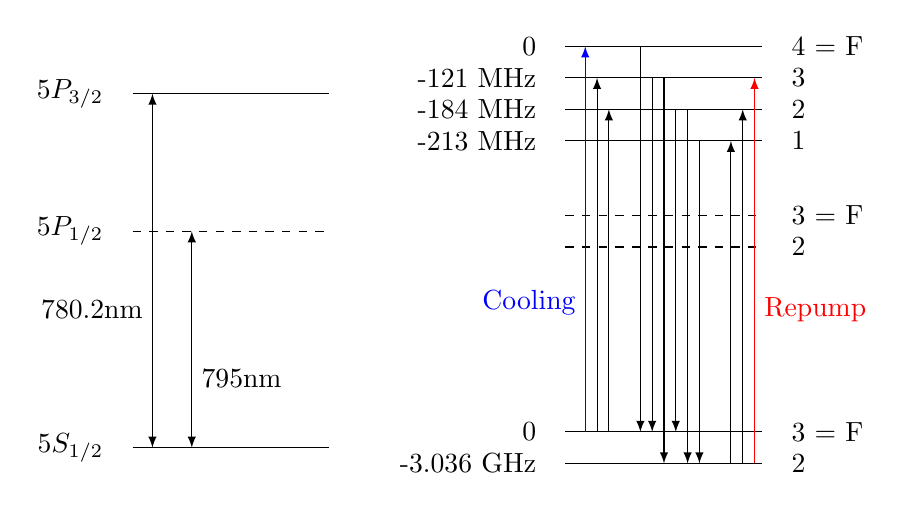
\begin{tikzpicture}[node distance=2.5cm]
        \node [label=left:\(5S_{1/2}\)] (Ground) {};
        \node [right=of Ground] (GroundHyper) {};

        \node [above=of Ground, label=left:\(5P_{1/2}\)] (D1) {};
        \node [right=of D1] (D1Hyper) {};

        \node [above=1.5cm of D1, label=left:\(5P_{3/2}\)] (D2) {};
        \node [right=of D2] (D2Hyper) {};

        \draw (Ground)--(GroundHyper);
        \draw [dashed] (D1)--(D1Hyper);
        \draw (D2)--(D2Hyper);

        \draw [<->] ([xshift=0.5cm]Ground.west)--([xshift=0.5cm]D2.west)
            node [midway,left,yshift=-0.5cm]{780.2nm};

        \draw [<->] ([xshift=1cm]Ground.west)--([xshift=1cm]D1.west)
            node [midway,right,yshift=-0.5cm]{795nm};

        \node [right=of GroundHyper, yshift=0.2cm, label=left:{0}] (GroundF3) {};
        \node [right=of GroundHyper, yshift=-0.2cm, label=left:{-3.036 GHz}] (GroundF2) {};
        \node [right=of GroundF3, label=right:{3 = F}] (GroundF3End) {};
        \node [right=of GroundF2, label=right:{2    }] (GroundF2End) {};
        \draw (GroundF3)--(GroundF3End);
        \draw (GroundF2)--(GroundF2End);

        \node [right=of D1Hyper, yshift=0.2cm] (D1F3) {};
        \node [right=of D1Hyper, yshift=-0.2cm] (D1F2) {};
        \node [right=of D1F3, label=right:{3 = F}] (D1F3End) {};
        \node [right=of D1F2, label=right:{2    }] (D1F2End) {};
        \draw [dashed] (D1F3)--(D1F3End);
        \draw [dashed] (D1F2)--(D1F2End);

        \node [right=of D2Hyper, yshift=0.6cm, label=left:{0}] (D2F4) {};
        \node [right=of D2F4, label=right:{4 = F}] (D2F4End) {};
        \node [right=of D2Hyper, yshift=0.2cm, label=left:{-121 MHz}] (D2F3) {};
        \node [right=of D2F3, label=right:{3}] (D2F3End) {};
        \node [right=of D2Hyper, yshift=-0.2cm, label=left:{-184 MHz}] (D2F2) {};
        \node [right=of D2F2, label=right:{2}] (D2F2End) {};
        \node [right=of D2Hyper, yshift=-0.6cm, label=left:{-213 MHz}] (D2F1) {};
        \node [right=of D2F1, label=right:{1}] (D2F1End) {};
        \draw (D2F4)--(D2F4End);
        \draw (D2F3)--(D2F3End);
        \draw (D2F2)--(D2F2End);
        \draw (D2F1)--(D2F1End);

        \draw [color=blue, ->] ([xshift=0.5cm]GroundF3.west)--([xshift=0.5cm]D2F4.west)
            node [midway, left, yshift=-0.8cm] {Cooling};
        \draw [->] ([xshift=0.65cm]GroundF3.west)--([xshift=0.65cm]D2F3.west);
        \draw [->] ([xshift=0.8cm]GroundF3.west)--([xshift=0.8cm]D2F2.west);

        \draw [->] ([xshift=1.2cm]D2F4.west)--([xshift=1.2cm]GroundF3.west);
        \draw [->] ([xshift=1.35cm]D2F3.west)--([xshift=1.35cm]GroundF3.west);
        \draw [->] ([xshift=1.5cm]D2F3.west)--([xshift=1.5cm]GroundF2.west);
        \draw [->] ([xshift=1.65cm]D2F2.west)--([xshift=1.65cm]GroundF3.west);
        \draw [->] ([xshift=1.8cm]D2F2.west)--([xshift=1.8cm]GroundF2.west);
        \draw [->] ([xshift=1.95cm]D2F1.west)--([xshift=1.95cm]GroundF2.west);
        
        \draw [->] ([xshift=2.35cm]GroundF2.west)--([xshift=2.35cm]D2F1.west);
        \draw [->] ([xshift=2.5cm]GroundF2.west)--([xshift=2.5cm]D2F2.west);
        \draw [color=red, ->] ([xshift=2.65cm]GroundF2.west)--([xshift=2.65cm]D2F3.west)
            node [midway, right, yshift=-0.5cm] {Repump};
    \end{tikzpicture}
    \caption{Diagram of the allowed transitions for rubidium-85.~\cite{ust}}
\end{figure}
\subsubsection{Closed optical loops, forbidden transitions, and dark states, oh my!}
We would love to have a simple two-state atom to perform optical cooling on; unfortunately, this is not possible in practice due to hyperfine splitting. The easiest atomic structure to cool is one that has a so-called ``closed optical loop''; that is,
an excitation-emission event that always returns an atom to its original state, ready to absorb another identical photon. Rubidium-85 has such a transition between the \(5S_{1/2},\,F=3\) state and the \(5P_{3/2},\,F=4\) state, since every other possible decay is a ``forbidden transition''.

Not every pair of source and destination energy levels forms a valid transition. According to selection rules such as conservation of angular momentum and parity, only a small subset are allowed by quantum mechanics. Take an atom in the excited \(5P_{3/2},\,F=4\) state.
It is prevented from decaying to any of the \(5P_{1/2}\) states because the spin would change direction, violating parity~\cite{harandbert}. It also cannot decay to the \(5S_{1/2},\,F=2\) state, since this would require an angular momentum change of -2, and a photon carries
a spin of 1. Thus, it can \textit{only} decay back to the \(5S_{1/2},\,F=3\) state, forming a closed optical loop.

In practice, lasers must be detuned from resonance to allow for Doppler cooling. This has the unfortunate complication of placing the frequency in an overlap between the \(5P_{3/2},\,F=4\) and the \(5P_{3/2},\,F=3\) states, meaning there is a small but nonzero probability that an
excited atom will arrive at a state that does \textit{not} form a closed optical loop. While an atom in this state still cannot decay to any of the \(5P_{1/2}\) states, it \textit{can} decay to the \(5S_{1/2},\,F=2\) state, since this requires an angular momentum change of only -1.
The cooling laser cannot excite an atom in this state, so we call it a ``dark state''. This would prevent further cooling of the atom if a repumping laser was not employed at the frequency needed to excite the atom back to the \(5P_{3/2},\,F=3\) state.
\subsection{Saturated absorption spectroscopy}
Absorption spectroscopy is theoretically straightforward. Given a gas of atoms with a transition of frequency \(f\), a laser scanning through a range of frequencies between \(f\pm\Delta f\) for some \(0<\Delta f<f\) will excite atoms when it is in the vicinity of \(f\). This causes a
reduction in the measured intensity of the beam \(I\). Plotting \(I\) as a function of \(f\) reveals all transitions of the atom in the scanned range.

Unfortunately, since the atoms in the gas are undergoing random thermal motion, a wider range of frequencies will be absorbed by the atoms. This tends to obscure more subtle features of absorption spectra, such as hyperfine splitting, in a process known as Doppler broadening. To overcome this, two antiparallel beams are used; a strong ``pump''
beam, and a weaker ``probe'' beam. The treatment here follows that of~\cite{satspec}.

Consider a gas of atoms with resonant frequency \(f\) and the distribution of velocities from Equation 1, with a pump beam travelling towards \(+\vec{\hat{x}}\) and a probe beam travelling towards \(-\vec{\hat{x}}\). If these beams have a frequency \(f_s<f\), the pump beam will interact only with
atoms travelling towards \(-\vec{\hat{x}}\), and the probe beam will interact only with atoms travelling towards \(\vec{\hat{x}}\). The opposite occurs if \(f_s>f\).
\begin{figure}[h]
    \centering
    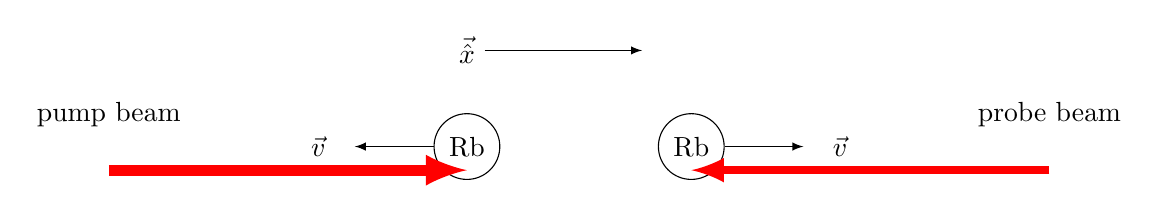
\begin{tikzpicture}[node distance=2cm]
        \node [draw, circle] (A) {Rb};

        \node [draw, circle, right=of A] (B) {Rb};

        \node [above=0.5cm of A] (AxisArrowStart) {\(\vec{\hat{x}}\)};
        \node [right=of AxisArrowStart] (AxisArrowEnd) {};
        \draw [->] (AxisArrowStart)--(AxisArrowEnd);

        \node [label=above:pump beam, left=4cm of A] (LeftLaserStart) {};
        \node [label=above:probe beam, right=4cm of B] (RightLaserStart) {};
        \draw [->, color=red, line width=4pt] ([yshift=-0.3cm]LeftLaserStart.center)--([yshift=-0.3cm]A.center);
        \draw [->, color=red, line width=3pt] ([yshift=-0.3cm]RightLaserStart.center)--([yshift=-0.3cm]B.center);
        \node [right=1cm of B, label=right:\(\vec{v}\)] (BArrowEnd) {};
        \node [left=1cm of A, label=left:\(\vec{v}\)] (AArrowEnd) {};
        \draw [->] (A)--(AArrowEnd);
        \draw [->] (B)--(BArrowEnd);
    \end{tikzpicture}
    \caption{Behaviour of the system when the probe and pump beams are off resonance.}    
\end{figure}

If instead \(f_s\approx f\), these two beams will both interact with only those atoms for which their velocity \(\vec{v}\cdot\vec{\hat{x}}\approx 0\). Importantly, both beams are interacting with the same set of atoms. The atoms are considered ``saturated'' if approximately half of them are in the
excited state at any time. Given this condition, many of the atoms will be in the excited state due to the pump beam, and will therefore not be able to absorb photons from the resonant probe beam. This manifests as a sharp decrease in absorption around the hyperfine transition frequencies of the atoms of interest.
\begin{figure}[h]
    \centering
    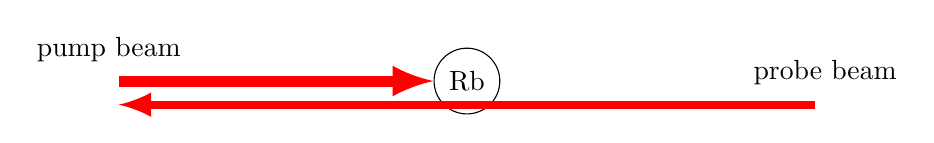
\begin{tikzpicture}[node distance=2cm]
        \node [draw, circle] (A) {Rb};
        \node [label=above:pump beam, left=4cm of A] (LeftLaserStart) {};
        \draw [->, color=red, line width=4pt] (LeftLaserStart)--(A);
        \node [label=above:probe beam, right=4cm of A, yshift=-0.3cm] (RightLaserStart) {};
        \node [left=4cm of A, yshift=-0.3cm] (RightLaserEnd) {};
        \draw [->, color=red, line width=3pt] (RightLaserStart)--(RightLaserEnd);
    \end{tikzpicture}
    \caption{Behaviour of the system when the probe and pump beams are on resonance.}
\end{figure}
\subsubsection{Crossover peaks}
A wrinkle that shows up in saturated absorption spectroscopy experiments is caused by an effect known as a ``crossover peak''. These tend to be much stronger than the actual hyperfine peaks, and are caused by interactions with atoms travelling at pathological velocities.

Consider an atom travelling at a velocity \(v\) with a gap between two transitions separated by frequency \(\Delta f\), where \(v\) is such that the pump beam Doppler shifted by \(\frac{\Delta f}{2}\). The probe beam will then be Doppler shifted by \(-\frac{\Delta f}{2}\). If the beams are at a frequency exactly halfway
between the transitons, both the pump and probe beams will be seen as on resonance, even though the frequency does not match any individual transiton. In practice, this means that small adjustments should be made to visible peaks to match the actual resonant frequency.
\subsection{The Zeeman effect}
Typical atomic energy levels have degeneracy; there are multiple possible configurations at the same energy level. These vary in the direction of the magnetic moments, so an external magnetic field causes these energy levels to split into three --- a higher energy level, a lower energy level, and the original level.
\subsection{Combined effects forming a MOT}
If we use two electromagnetic coils in anti-Helmholtz configuration, their magnetic field forms a magnetic quadrupole field\footnote{For a really cool animated version, see \url{http://tinyurl.com/y8zkkagb}.}, with a strength directly proportional to distance from their shared centre. Atoms that are further from this centre therefore experience stronger Zeeman splitting; their energy levels move closer to
the detuned laser's resonance, and they are therefore more likely to interact with the cooling laser. This results in a net restorative force towards the trap's centre.
\begin{figure}[h]
    \centering
    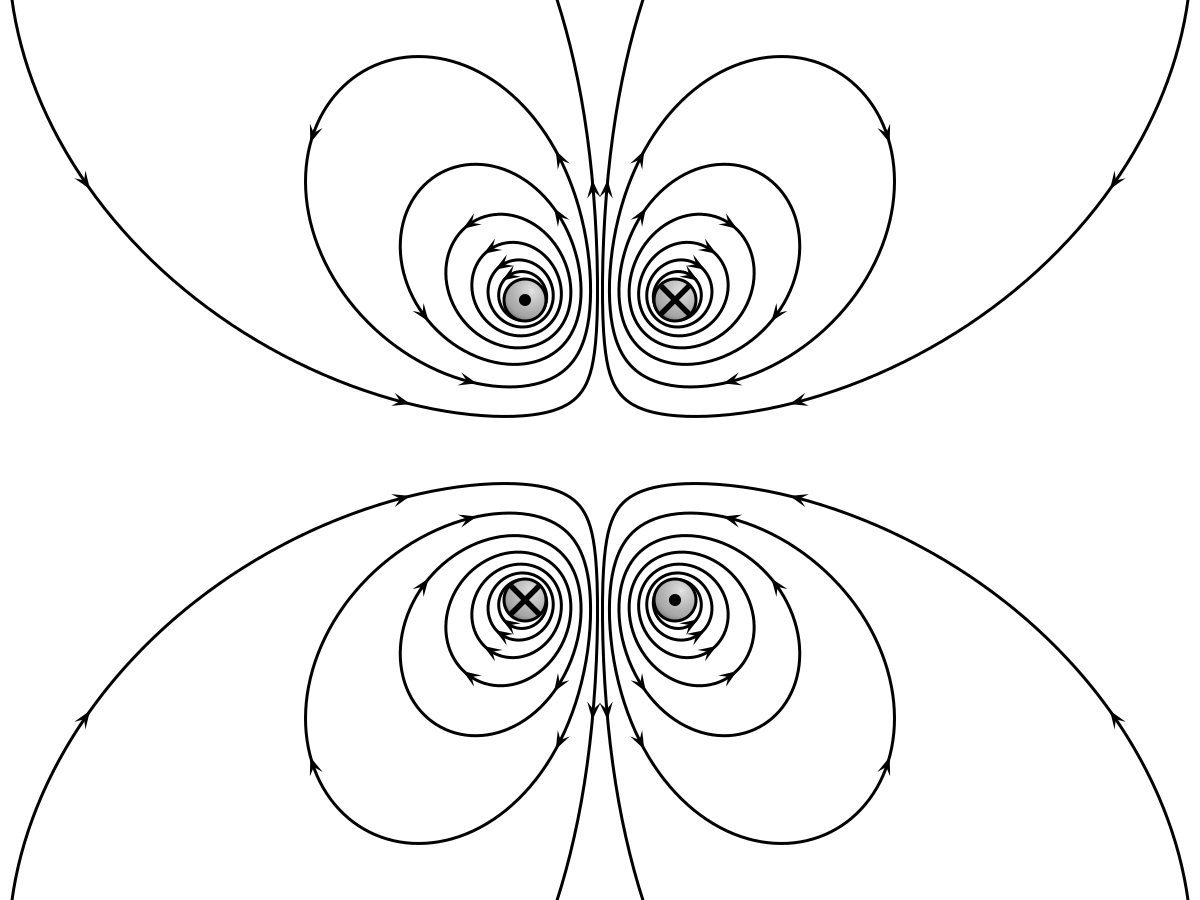
\includegraphics[width=0.5\textwidth]{images/quadrupole.png}
    \caption{
        A sketch of the field lines of a magnetic quadrupole.
    \cite{wikiquad}}
\end{figure}

A subtlety is introduced by the Zeeman-shifted levels' dependence on polarisation. The lower energy level accepts only left-circularly polarised (\(\sigma^-\)) light, and the upper energy level accepts only right-circularly polarised light (\(\sigma^+\)) (defined relative to the magnetic field). For atoms to be trapped, we need to shift the lower energy
levels closer to the beam's resonance, but only for those atoms \textit{towards} the beam. Fortunately, on opposite sides of the field, the magnetic field has the opposite sign; therefore, the needed polarisation is reversed, and atoms on the opposite side to the beam's source are not affected.~\cite{umkc}
\begin{figure}[h]
    \centering
    \begin{subfigure}{.3\textwidth}
        \centering
        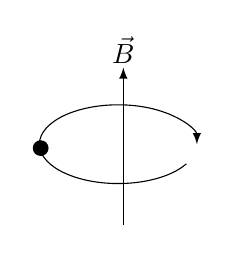
\begin{tikzpicture}[node distance=2cm]
            \node (Bbase) {};
            \node [above=of Bbase] (Btip) {};
            \draw [->] (Bbase)--(Btip)
                node [near end, yshift=0.3cm, label=above:{\(\vec{B}\)}] {};
            \draw [->] (0.8cm,0.9cm) arc [start angle=330, end angle=0, x radius=1cm, y radius=0.5cm];
            \fill (-1.05,1.1) circle (0.1cm);
        \end{tikzpicture}
        \caption{\(\sigma^-\) polarisation (lower level)}
    \end{subfigure}
    \begin{subfigure}{.3\textwidth}
        \centering
        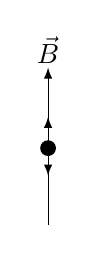
\begin{tikzpicture}[node distance=2cm]
            \node (Bbase) {};
            \node [above=of Bbase] (Btip) {};
            \draw [->] (Bbase)--(Btip)
                node [near end, yshift=0.3cm, label=above:{\(\vec{B}\)}] {};
            \draw [<->] ([yshift=0.75cm]Bbase.center)--([yshift=-0.75cm]Btip.center);
            \fill (0,1.1) circle (0.1cm);
        \end{tikzpicture}
        \caption{\(\pi\) polarisation (unshifted level)}
    \end{subfigure}
    \begin{subfigure}{.3\textwidth}
        \centering
        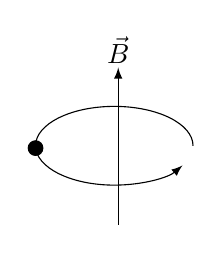
\begin{tikzpicture}[node distance=2cm]
            \node (Bbase) {};
            \node [above=of Bbase] (Btip) {};
            \draw [->] (Bbase)--(Btip)
                node [near end, yshift=0.3cm, label=above:{\(\vec{B}\)}] {};
                \draw [->] (0.95cm,1.13cm) arc [start angle=0, end angle=330, x radius=1cm, y radius=0.5cm];
                \fill (-1.05,1.1) circle (0.1cm);
        \end{tikzpicture}
        \caption{\(\sigma^+\) polarisation (higher level)}
    \end{subfigure}

    \caption{Sign convention for Zeeman-shifted levels' polarisation.}
\end{figure}
\vfill
\pagebreak
\section{Experimental procedure}
\subsection{External-cavity diode lasers}
The heart and soul of the experiment was two external-cavity diode lasers (ECDLs). The design uses a laser diode
with a high-reflectivity rear surface, and a low-reflectivity front surface; the lasing is instead performed by reflections
from a diffraction grating placed approximately 20mm in front of the diode.~\cite{moglabsecd} An additional mirror is used to counteract
the angular displacement from the diffraction grating.
\begin{figure}[h]
    \centering
    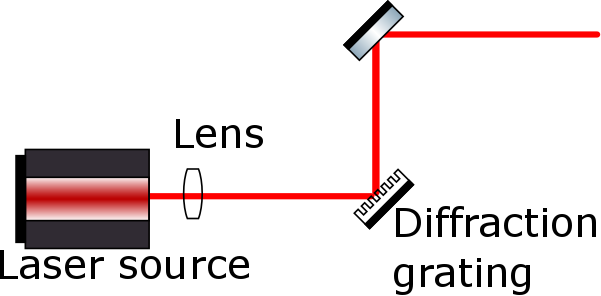
\includegraphics[width=.3\textwidth]{images/ecdl-internals.png}
    \caption{Diagram of the laser internals.}
\end{figure}

A piezoelectric transducer (PZT) rests against the diffraction grating to allow for scanning of the laser's frequency by sending a
triangle wave to the PZT.\@ This is provided by a MOGLabs diode laser controller, providing the ability to precisely control the range
and midpoint of this scan by changing the current of the diode, as well as a frequency offset.

We used one laser emitting approximately 90 mW of laser power as the cooling laser, and another emitting approximately 27.3 mW as the
repumping laser. Since the cooling beam was split into three pieces, it needed to have a much higher power than the repumping laser.
\subsection{Absorption spectroscopy}
The first thing that needs to be done to create the MOT is to ensure the lasers can be tuned accurately to hyperfine transitions. As a
first stepping stone, we built a simple absorption spectroscopy setup.
\begin{figure}[h]
    \centering
    \caption{Diagram of the basic absorption spectroscopy bench.}
\end{figure}

Our first effort did not use the isolators or waveplate. We found first that the photodiode was oversaturated with power, so the waveplate
was added to allow changing the beam balance through the PBS.\@
\subsection{Saturated absorption spectroscopy}
\subsection{Vacuum cell setup}
\subsection{Magnetic quadrupole}
\subsection{Arrangement for optical molasses}
\subsection{Fine-tuning to create the trap}
\section{Results and discussion}
\section{Future work}
\vfill
\pagebreak
\section{References}
\bibliography{papers}
\bibliographystyle{unsrt}
\end{document}